\documentclass{beamer}
\usepackage{graphicx}
\graphicspath{{./images/}}

%Information to be included in the title page:
\title{Mathematics in Deep Learning}
\author{Lachlan Jones}
\institute{Math199}
\date{2024}

\usecolortheme{beaver}
% \setbeamertemplate{navigation symbols}{}

\begin{document}

\frame{\titlepage}

\begin{frame}
    \frametitle{Deep Learning, over-simplified}
    Matching a trend to some data:
    \begin{figure}
        \centering
        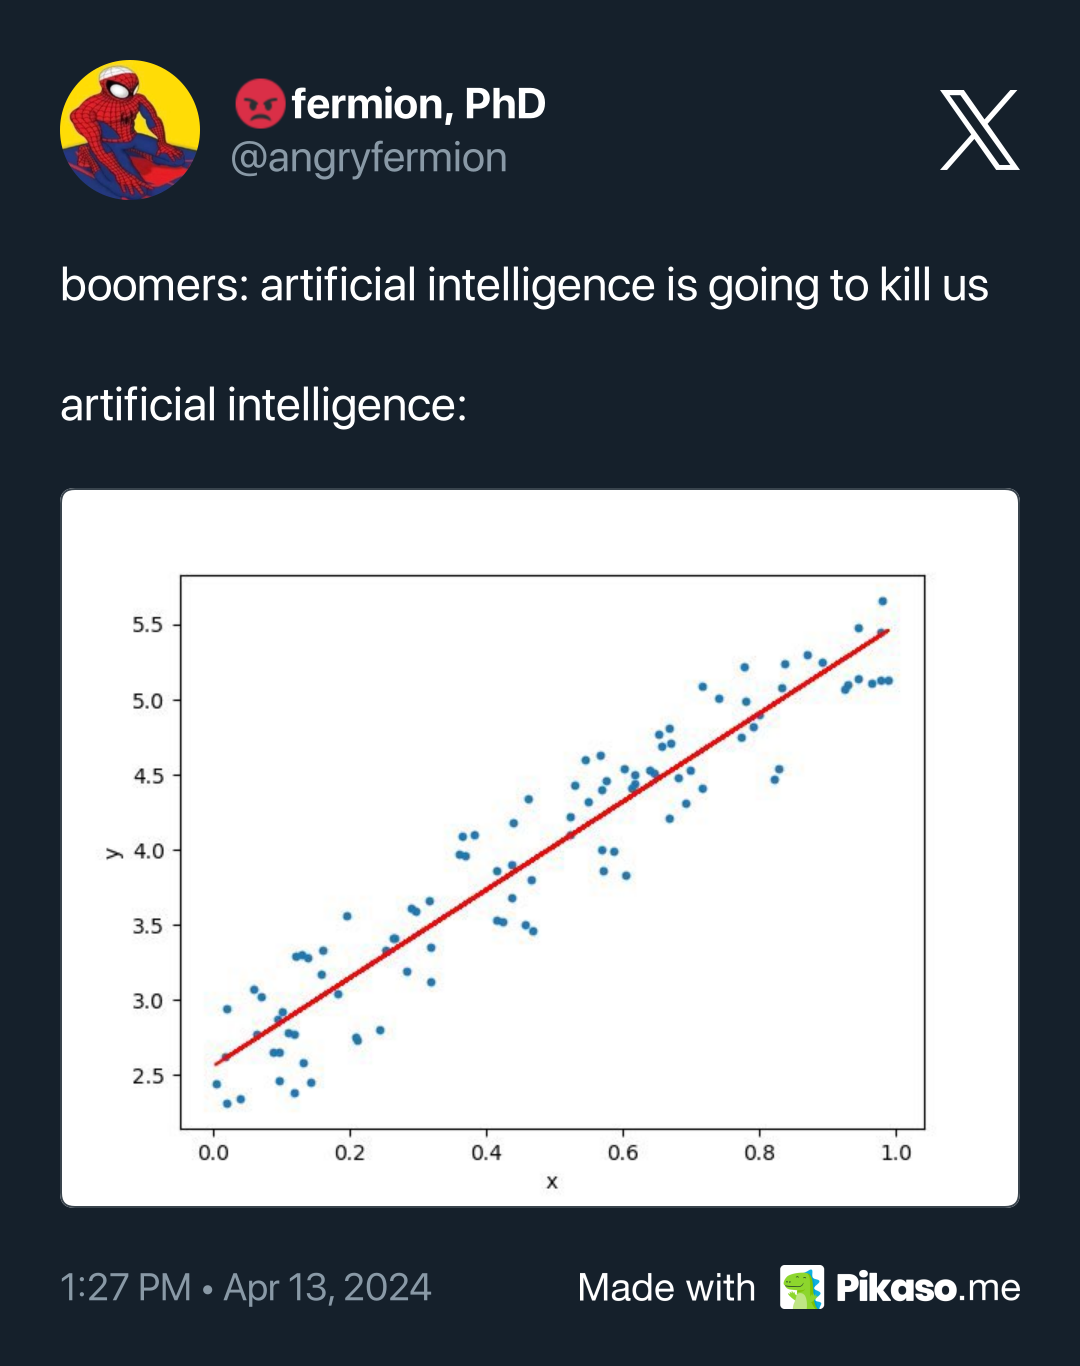
\includegraphics[height=0.75\textheight]{pikaso.me-angryfermion-20240413_132756-1779139460174676132.png}
    \end{figure}
\end{frame}

\begin{frame}
    \frametitle{Perceptrons, the building block of Neural Networks}
\end{frame}

% \begin{frame}
%     \frametitle{Sample frame title}
%     This is a text in second frame.
%     For the sake of showing an example.

%     % \begin{itemize}
%     %     \item<1-> Text visible on slide 1
%     %     \item<2-> Text visible on slide 2
%     %     \item<3> Text visible on slide 3
%     %     \item<4-> Text visible on slide 4
%     % \end{itemize}
%     \begin{itemize}
%         \item Text visible on slide 1 \pause
%         \item Text visible on slide 2 \pause
%         \item Text visible on slide 3 \pause
%         \item Text visible on slide 4
%     \end{itemize}
% \end{frame}

\end{document}